
\chapter{Preliminary Results}
\graphicspath{{Preliminary Results/Vector/}{Preliminary Results/}}

The proposed SAR ADC architecture is being studied, researched, and simulated. So far, the bootstrapped T/H switch, and the StrongARM Latch have been simulated in Cadence Virtuoso tool. The channel has also been statistically modelled by including the effect of ADC's quantization noise in a SerDes link using MATLAB. The results are following sections.

%%%%%%%%%%%%%%%%%
%%%%%%%%%%%%%%%%%%
%%%%%% Chapter 4 Section 1
%%%%%%%%%%%%%%%%%
%%%%%%%%%%%%%%%%%%
\section{Time Domain Analysis of SerDes Link}

A RPBS sequence was generated and passed through an AWGN channel in a SerDes wireline channel. The eye diagram of the channel response was plotted as shown in Figure 4.1. \\

\begin{figure*}[h]
	\centering
	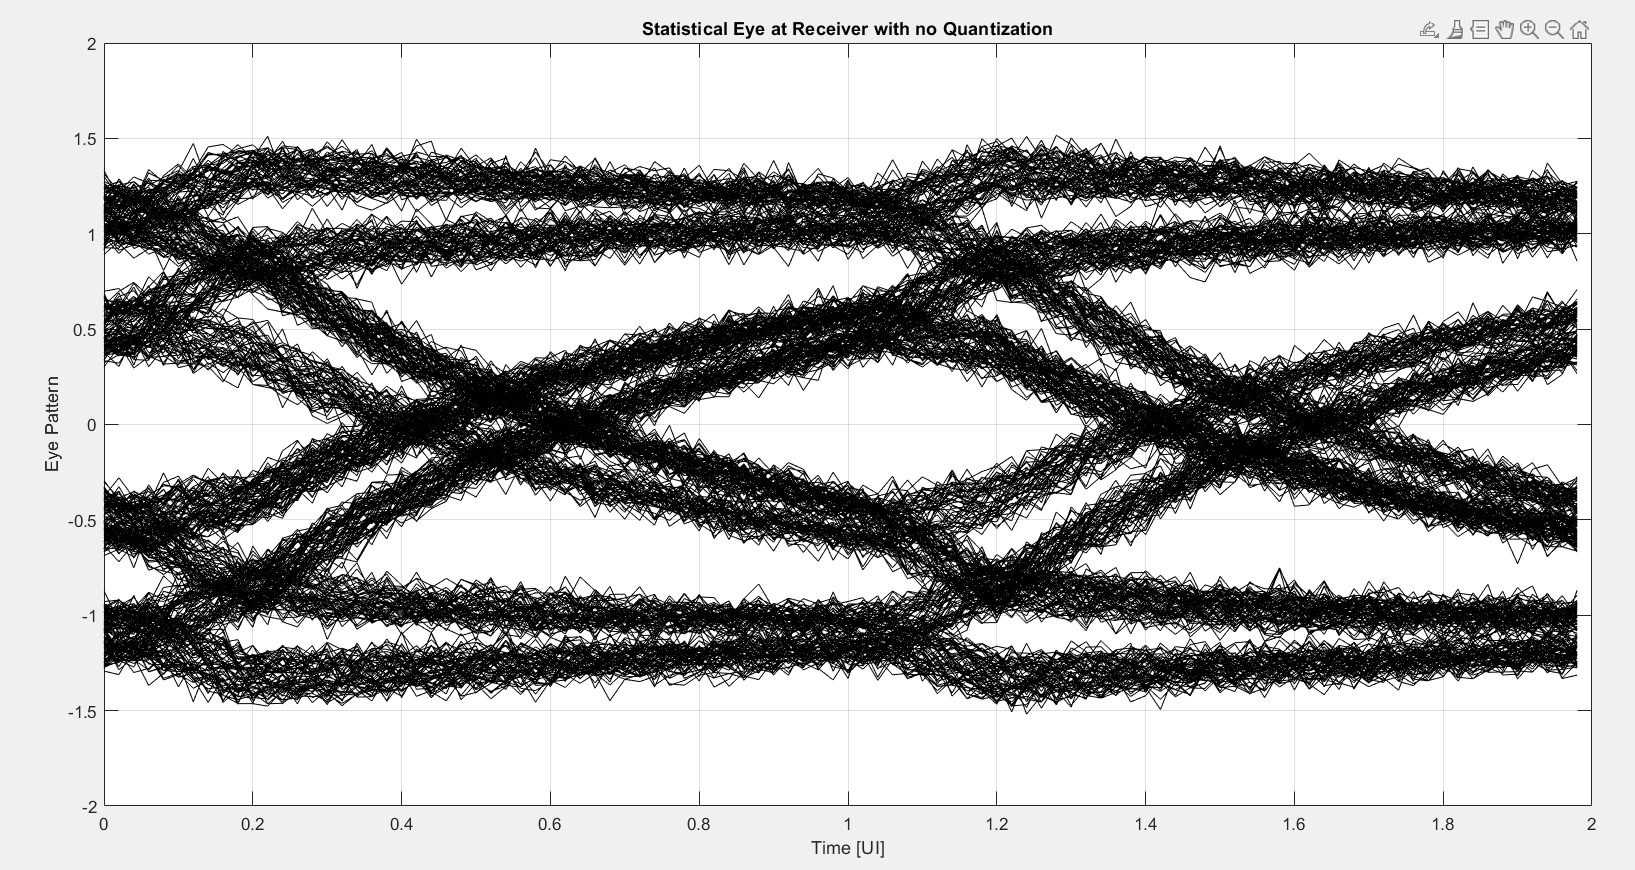
\includegraphics[width=12cm,height=6cm]{fig4_1.png}
	\caption{Statistical Eye with no Quantization}
	\label{eye_wo_q}
\end{figure*}

Next, quantization was added to the channel response in order to see the effect of including an ADC in the receiver. The waveforms clearly  shows that an open eye can be achieved with a quantization of about 5-6 bits and nothing lower than that. The eye diagrams for quantization with 8, 5, and 3 bits have been plotted in Figure 4.2 to understand this phenomena.

\begin{figure*}[h]
	\centering
	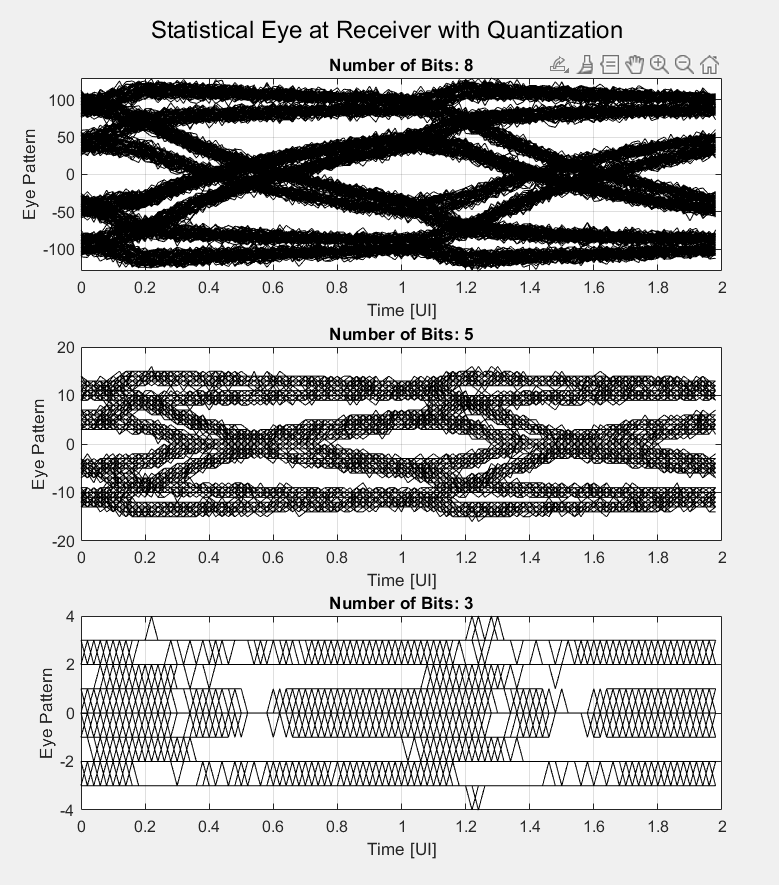
\includegraphics[width=12cm,height=12cm]{fig4_2.png}
	\caption{Statistical Eye with Quantization}
	\label{eye_w_q}
\end{figure*}


\section{Design of Sub-ADC}
\rhead{Design of Sub-ADC}
\label{Design of Sub-ADC}

\subsection{Bootstrapped switch}

A simple bootstrapped switch has been designed and simulated using the Cadence Virtuoso tool with $USMC\; 65\,nm$ PDK. The sampling frequency was chosen to be \textbf{$1\: GHz$} and the message signal frequency was chosen to be \textbf{$125\: MHz$}. The resulting waveform can be seen in the Figure 4.3. Very little non-idealities and non-linearities can be observed which are negligible.

\begin{figure*}[h]
	\centering
	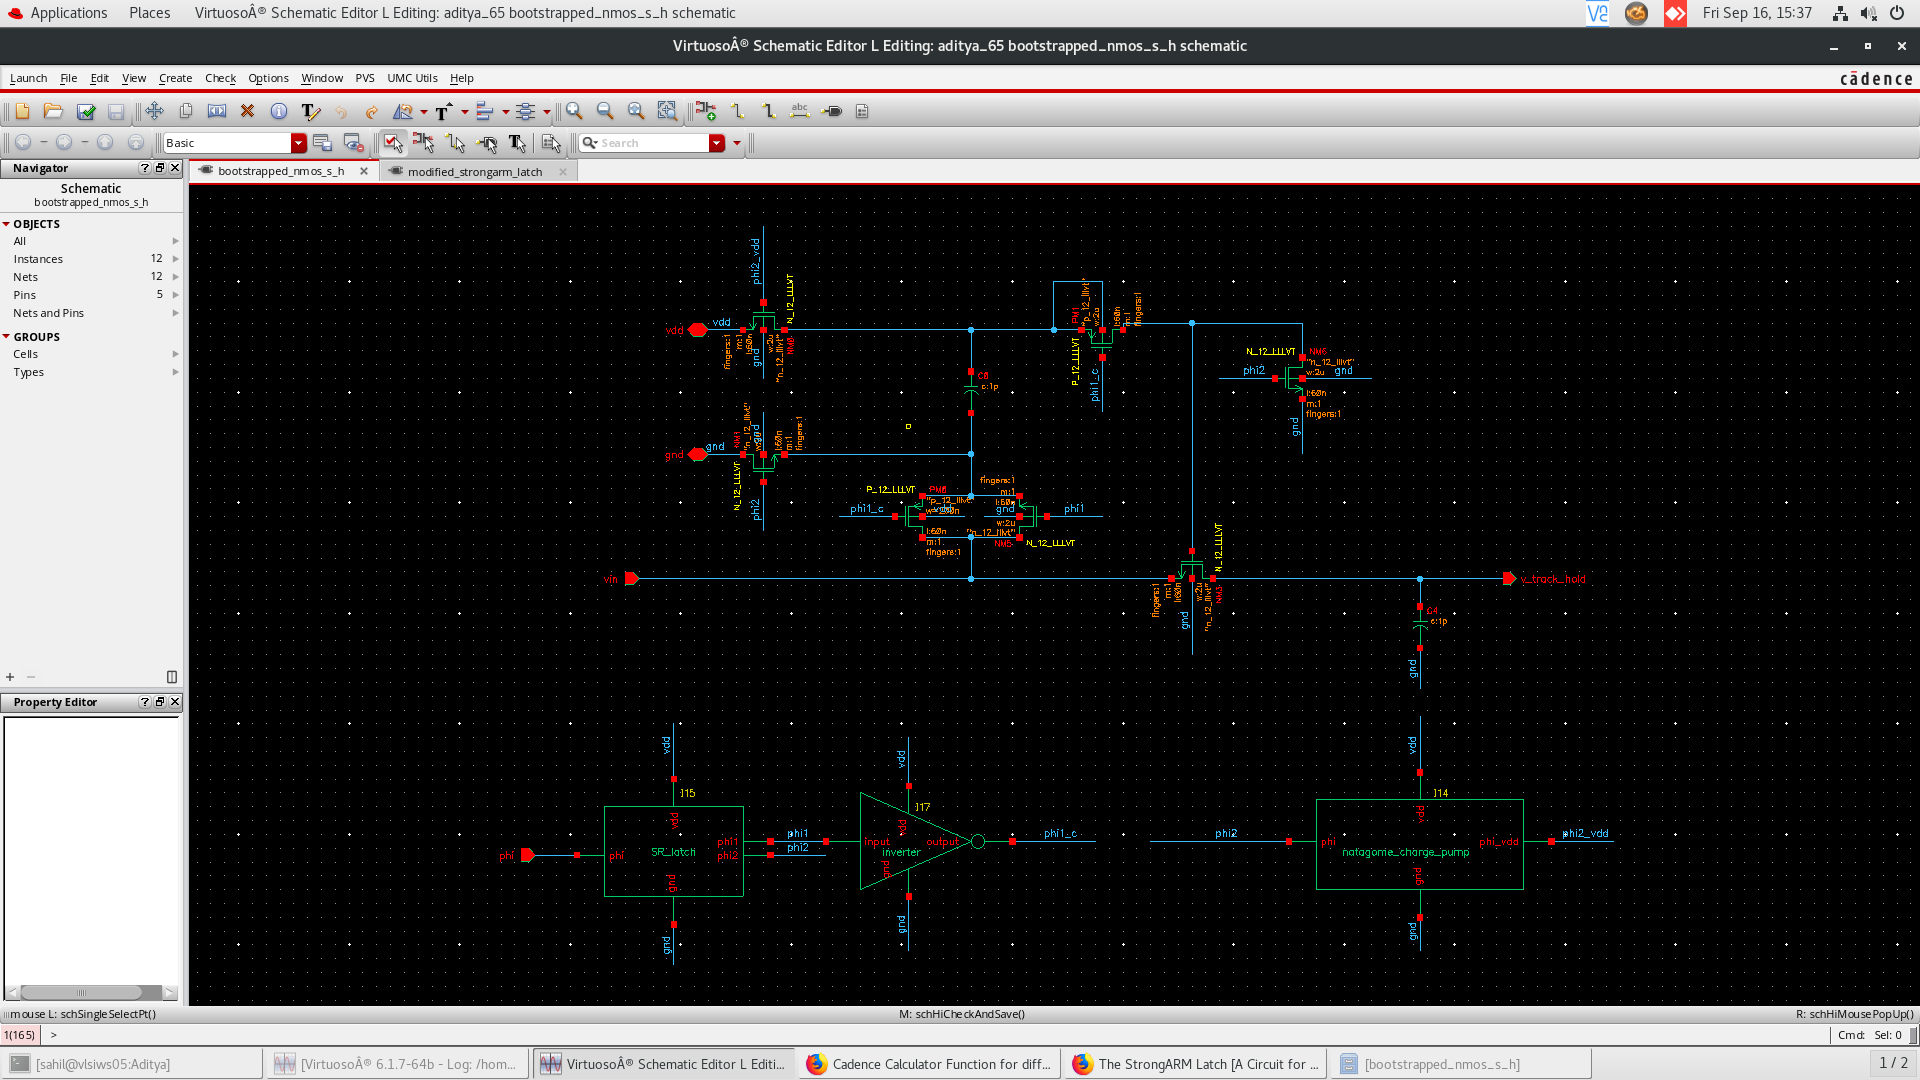
\includegraphics[width=16cm,height=8cm]{fig4_3.png}
	\caption{Bootstrapped Track and Hold Circuit Schematic}
	\label{t_h_ckt}
\end{figure*}

\begin{figure*}[h]
	\centering
	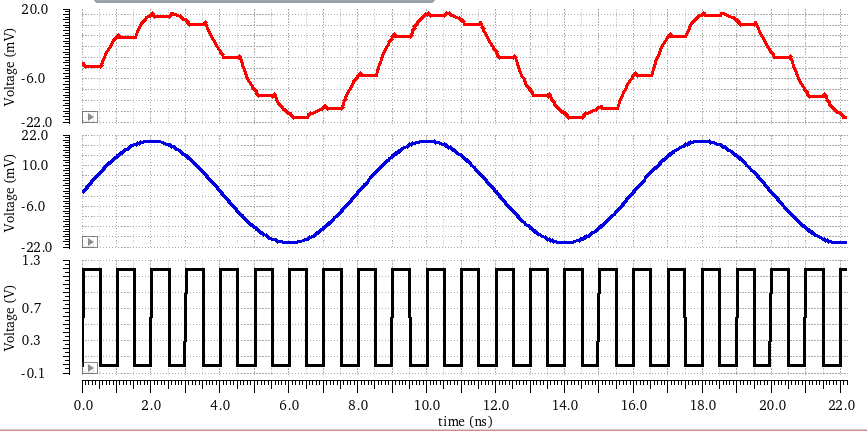
\includegraphics[width=16cm,height=8cm]{fig4_4.png}
	\caption{Bootstrapped Track and Hold Waveform}
	\label{t_h_waveform}
\end{figure*}

\subsection{StrongARM Latch}

A StrongARM Latch has also been simulated using Cadence Virtuoso tool in $USMC\! 65 \, nm$ PDK. The \textbf{Clock} was a pulse with a period of \textbf{1 GHz}. The input \textbf{$V_{in1}$} was \textbf{grounded}, whereas the input \textbf{$V_{in2}$} was connected to \textbf{$V_{DD}$}. The output clearly shows \textbf{$V_{x}$} reaches an output voltage of \textbf{$V_{DD}$}, while \textbf{$V_{y}$} settles to 0 voltage after a while within the clock cycle. 

\begin{figure*}[h]
	\centering
	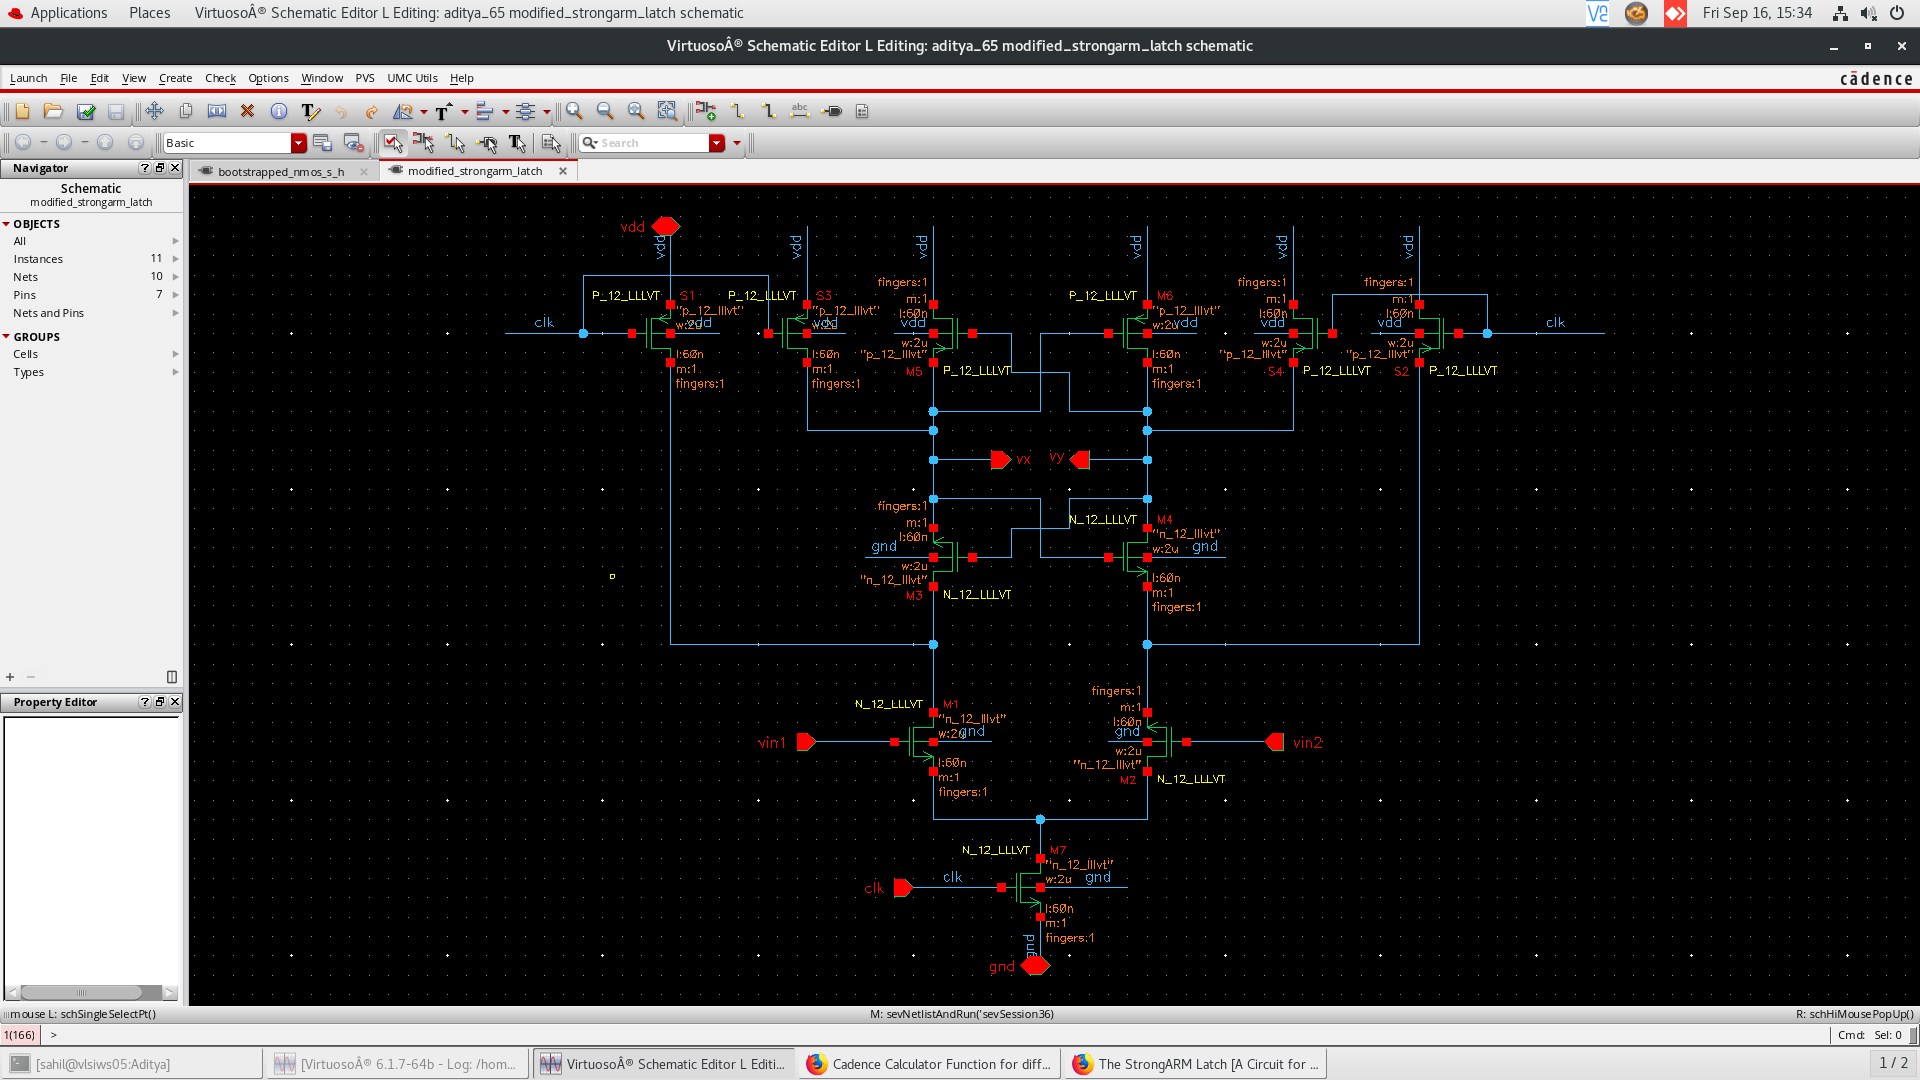
\includegraphics[width=16cm,height=8cm]{fig4_5.png}
	\caption{StrongARM Latch Circuit Schematic}
	\label{comp_ckt}
\end{figure*}

\begin{figure*}[h]
	\centering
	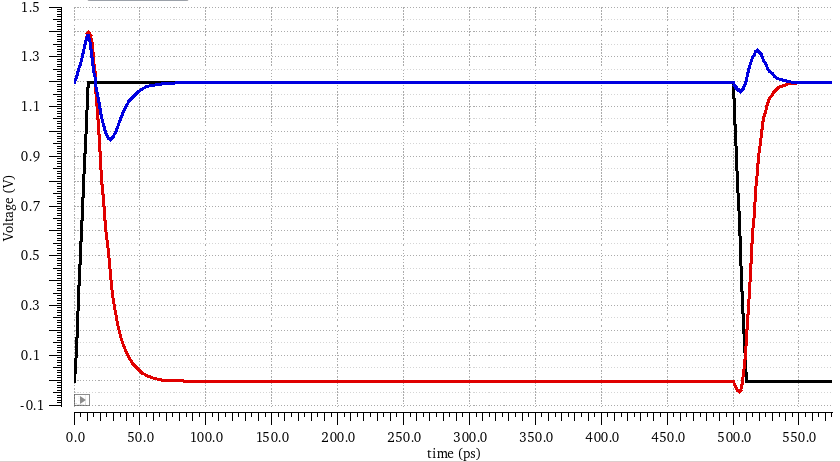
\includegraphics[width=16cm,height=8cm]{fig4_6.png}
	\caption{StrongARM Latch Output Waveform}
	\label{comp_waveform}
\end{figure*}

Another latch circuit has also been designed by clocking the differential pair through the cross-coupled NMOS pair in order to have a low kick-back current through the circuit when the circuit is in idle state. Its results can be seen in Figures 4.7-8. We can see that in the case of low kick-back circuit, the output voltages have more controlled peaks and peak only upto $1.3\,V$, whereas in the earlier case, the output voltages (\textbf{$V_{x}\: and \: V_{y}$}) peaked upto $1.4\,V$.

\begin{figure*}[h]
	\centering
	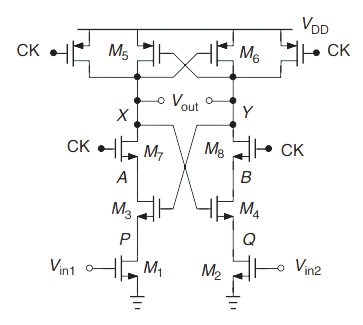
\includegraphics[width=12cm,height=8cm]{fig4_7.png}
	\caption{An alternative topology for lower kick-back noise [7]}
	\label{comp_lk_ckt}
\end{figure*}

\begin{figure*}[h]
	\centering
	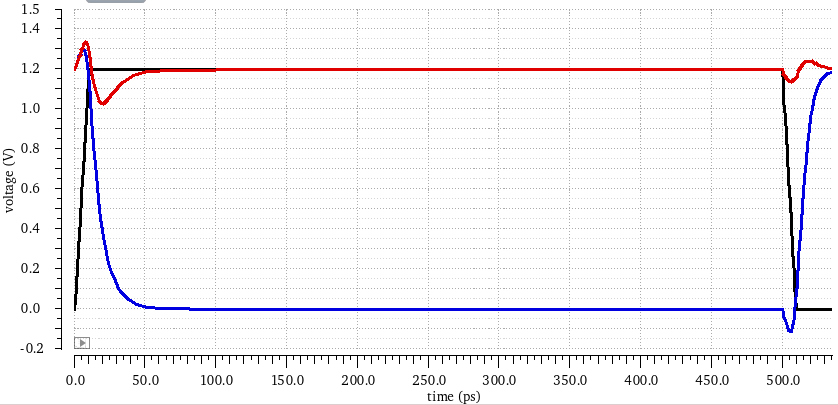
\includegraphics[width=16cm,height=8cm]{fig4_8.png}
	\caption{StrongARM Latch Low kick-back Output Waveform}
	\label{comp_lk_waveform}
\end{figure*}
\newpage